\section{Semaine 19 (03/03 - 07/03) }


\e{Notions abordées :}
\begin{itemize}
	\item Régime sinusoïdal forcé.
	\item Filtrage linéaire.
\end{itemize}

\subsection{Questions de cours}

\begin{enumerate}
	\item Grandeur complexe associée à un signal sinusoïdal réel.
	\item Impédances des dipôles usuels. Démonstration.
	\item Exprimer le signal de sortie d'un filtre linéaire en notation réelle en fonction de la fonction de transfert.
\end{enumerate}

\subsection{Exercice 1 : Circuit $RLC$ parallèle et anti-résonance}

On considère le circuit suivant où le générateur délivre une tension sinusoïdale $e(t)$ d'amplitude $e_m$.

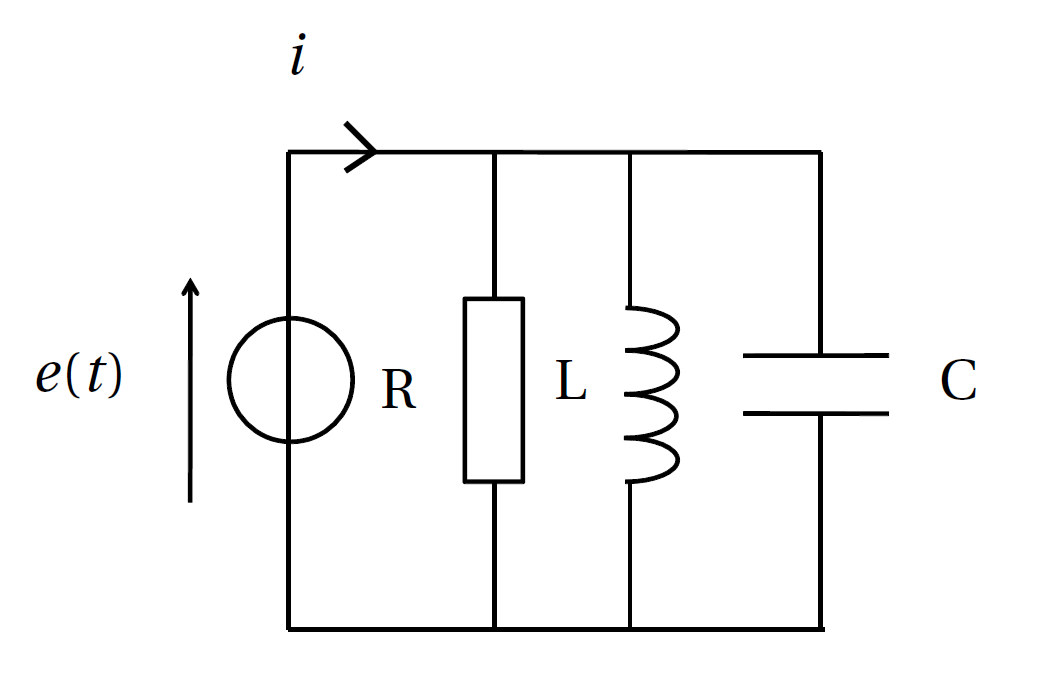
\includegraphics[width = \textwidth]{./Images/mpsi_s19_ex01.png}

\begin{enumerate}
	\item Exprimer l'impédance équivalente de l'association des trois dipôles en fonction de $C$, $L$, $R$ et $\omega$.
	\item Montrer que l'amplitude $i_m$ du courant admet un minimum en fonction de $\omega$ pour une certaine pulsation $\omega_0$ à déterminer en fonction de $L$ et $C$.
	\item Quel serait le facteur de qualité $Q$ du circuit ?
\end{enumerate}

\subsection{Exercice 2 : Caractère dérivateur d'un filtre}

On considère le circuit suivant : 

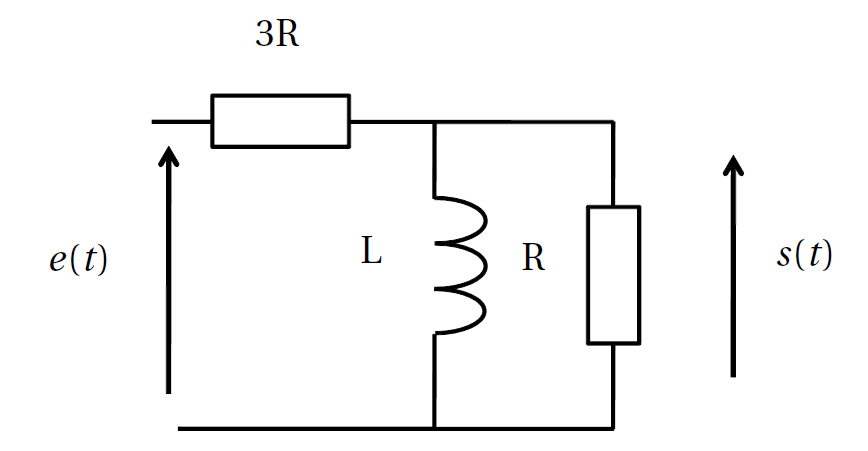
\includegraphics[width = \textwidth]{./Images/mpsi_s19_ex02.png}

On donne $L = \SI{20}{mH}$ et $R = \SI{5.0}{\kilo\ohm}$.

\begin{enumerate}
	\item Prédire sans calcul la nature du filtre.
	\item Déterminer sa fonction de transfert. La mettre sous forme canonique.
	\item Tracer le diagramme de Bode en gain et en phase.
	\item Montrer que ce filtre a un caractère dérivateur en basses fréquences.
	\item On envoie en entrée un signal $e(t) = 5 + 4\sin(2\pi f_1 t -2.0)$ avec $f_1 = \SI{80}{kHz}$. Déterminer l'expression de $s(t)$.
	\item Indiquer qualitativement l'effet de ce filtre sur un signal d'entrée de type créneau de fréquence $f = \SI{80}{kHz}$ oscillant entre $\SI{0.0}{V}$ et $\SI{8.0}{V}$.
	\item Indiquer qualitativement l'effet de ce filtre sur un signal d'entrée de type triangle de fréquence $f = \SI{80}{kHz}$ oscillant entre $\SI{-10}{V}$ et $\SI{10}{V}$.
\end{enumerate}

\subsection{Exercice 3 : Résonance d'un circuit bouchon}

On considère le circuit suivant avec $e(t) = e_m \cos \omega t$.

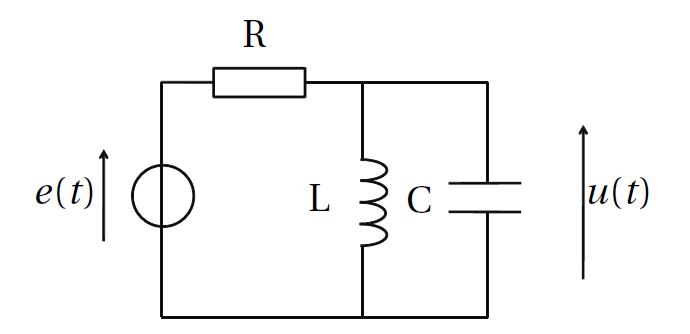
\includegraphics[width = \textwidth]{./Images/mpsi_s19_ex03.png}

\begin{enumerate}
	\item Quelle est l'impédance équivalente de l'association en parallèle de la capacité $C$ et de l'inductance $L$ ?
	\item Par la formule du pont diviseur de tensions déterminer l'amplitude complexe de $u$ en fonction de $R$, $C$, $\omega$, $L$ et $e_m$. Comment s'appelle l'expression ainsi déterminée ?
	\item Montrer qu'il apparaît une résonance. 
	\item Déterminer le facteur de qualité du système.
	\item Calculer numériquement la fréquence de résonance, le facteur de qualité et la largeur de la bande passante pour $R = \SI{1.0}{\kilo\ohm}$, $L = \SI{10}{mH}$ et $C = \SI{0.50}{\micro\farad}$.
	\item Montrer que le déphasage est une fonction décroissante de la fréquence. Calculer sa valeur pour $\omega = 0$, à la résonance et en très hautes fréquences. Tracer l'allure du déphasage en fonction de la fréquence.
\end{enumerate}
